\documentclass[a4paper, norsk, 8pt]{article}
\usepackage[utf8]{inputenc}
\usepackage[T1]{fontenc}
\usepackage{babel, textcomp, color, amsmath, amssymb, tikz, subfig, float,esint}
\usepackage{amsfonts}
\usepackage{physics}
\usepackage{graphicx}
\usepackage{multicol}
\usepackage{tikz}
\usepackage{pgfplots}

\newcommand{\EQU}[1] { \begin{equation*} \begin{split}
#1  
\end{split} \end{equation*} }
 \newcommand{\DE}[1] {  \begin{description}  #1 \end{description} }
 \newcommand{\IT}[2] { \item[\color{blue} #1]{#2} }
 \newcommand{\vv}[1] { \mathbf{#1} }
 \newcommand{\PAR}[2]{ \frac{\partial #1}{\partial #2}}
 \newcommand{\expe}[1] { \left\langle#1\right\rangle }
 \newcommand{\ket}[1] { |#1\rangle }
  \newcommand{\bra}[1] { \langle #1 | }
  \newcommand{\braket}[2] { \langle #1 | #2 \rangle }
  \newcommand{\commutator}[2]{ \left[ #1 , #2\right] }
  \newcommand{\colvec}[2] { 
  \left( \begin{matrix}
 #1 \\
 #2 \\
  \end{matrix}\right) }
 \newcommand{\PLOTS}[4]{ 
\begin{tikzpicture}
\begin{axis}[
    axis lines = #3, %usally left
    xlabel = #1,
    ylabel = #2,
]
#4
\end{axis}
\end{tikzpicture}
}


\newcommand{\addPLOT}[4]{
\addplot [domain=#1:#2,samples=200,color=#3,]{#4};}
\newcommand{\addCOORDS}[1]{\addplot coordinates {#1};}
\newcommand{\addDRAW}[1]{\draw #1;}
\newcommand{\addNODE}[2]{ \node at (#1) {#2};}

%		\PLOTS{x}{y}{left}{
%			\ADDPLOT{x^2}{-2}{2}{blue}
%			\ADDCOORDS{(0,1)(1,1)(1,2)}
%		}




\definecolor{svar}{RGB}{0,0,0}
\definecolor{opgavetekst}{RGB}{109,109,109}
\definecolor{blygraa}{RGB}{44,52,59}

\hoffset = -60pt
\voffset = -95pt
\oddsidemargin = 0pt
\topmargin = 0pt
\textheight = 0.97\paperheight
\textwidth = 0.97\paperwidth

\begin{document}
\tiny
\begin{multicols*}{2}
\subsubsection*{\scriptsize Solution exam 2018}
\subsubsection*{\scriptsize Exercise 1: Penalized regression}
\textbf{1a)}
\begin{figure}[H]
	\centering
	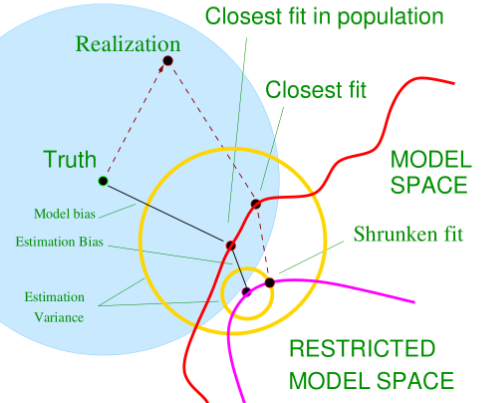
\includegraphics[width=0.2\textwidth]{bias_variance1.png}
\end{figure}   
Using the figure above, explain the concept of bias-variance trade-off\\
\textbf{ans:}When using the squared-error loss, the expected prediction error can be decomposed into three parts:
\begin{itemize}
	\setlength\itemsep{0.04em}
	\item an irreducible error, which cannot be avoided;
	\item the squared bias, where bias is the difference between the average of the estimate and the true mean;
	\item a variance term, the expected square deviation of our estimate from its mean
\end{itemize}
When minimizing the expected prediction error, we are in a situation in which if we reduce the variance component, for example by adding constraints to the model space, we increase the squared bias, and vice versa.  This is called bias-variance trade-off.  In the picture this is represented by lines and circles: when adding constraints, o.e. when we move from the model space to the restricted model space, we increase the bias (represented by the line named “Estimation Bias") but we reduce the variance (the radius of the circle around the “Closest fit in population” point is smaller than that around the corresponding point on the restricted model space\\
\textbf{1b)} Show analytically the same concept of the point above by mathematicallycomparing bias and variance of the ordinary least square estimator and ofthe ridge estimator\\
\textbf{ans:} bias:
\begin{align}
	E[\hat{\beta}_{OLS}] &= \beta\\
	E[\hat{\beta}_{ridge}] &= E[(X^TX + \lambda I)^{-1}X^Ty]\\
	 &= E[(\lambda I + \lambda(X^TX)^{-1})^{-1}(X^TX)^{-1}X^Ty]\\
	 &= E[(\lambda I + \lambda(X^TX)^{-1})^{-1}] E[\hat{\beta}_{OLS}]\\
	 &= w_\lambda \beta \Rightarrow E[\hat{\beta}_{ridge}]\neq \beta \text{ for } \lambda>0
\end{align}
variance:
\begin{align}
	Var[\hat{\beta}_{OLS}] &= \sigma^2 (X^TX)^{-1}\\
	Var[\hat{\beta}_{ridge}] &= Var[w_\lambda \hat{\beta}_{OLS}]\\
	&= w_\lambda Var[\hat{\beta}_{OLS}]w^T_\lambda\\
	&= \sigma^2 w_\lambda (X^TX)^{-1}w^T_\lambda.
\end{align}
then:
\begin{align}
	&Var[\hat{\beta}_{OLS}] - Var[\hat{\beta}_{ridge}] = \sigma^2[(X^TX)^{-1}-w_\lambda (X^TX)^{-1}w^T_\lambda]\\
	&=\sigma^2w_\lambda [(I+\lambda(X^TX)^{-1})(X^TX)^{-1}(I+\lambda(X^TX)^{-1})^T - (X^TX)^{-1}]w^T_\lambda\\
	&= \sigma^2w_\lambda [((X^TX)^{-1}+2\lambda(X^TX)^{-2}+\lambda^2(X^TX)^{-3})-(X^TX)^{-1}] w^T_\lambda\\
	&= \sigma^2w_\lambda [2\lambda(X^TX)^{-2}+\lambda^2(X^TX)^{-3}]w^T_\lambda > 0
\end{align}
(since all terms are quadratic and therefore positive)
\begin{equation}
	\Rightarrow Var[\hat{\beta}_{ridge}] \leq Var[\hat{\beta}_{OLS}]
\end{equation}
\subsubsection*{\scriptsize Exercise 2: Bootstrapping for model evaluation}
\textbf{2)} Bootstrapping for model selection. Consider the following procedure to estimate the prediction error:
\begin{enumerate}
	\item generate $B$ bootstrap samples $z_1,...,z_B$, where $z_b={(y^*_1,x^*_1),...,(y^*_N,x^*_N)}$, $b= 1,...,B$, and $(y^*_i,x^*_i),i= 1,...,N$ is an observation sampled from the original dataset;
	\item apply the prediction rule to each bootstrap sample to derive the predictions $\hat{f}^*_b(x_i)$, $b= 1,...,B$;
	\item compute the error for each point, and take the average:
\end{enumerate}
\begin{equation}
	\hat{\text{Err}_{\text{boot}}} = \frac1B\sum^B_{b=1}\frac1N \sum^N_{i=1}L(y_i,\hat{f}^*_b(x_i))
\end{equation}
\textbf{2a)}Explain why this procedure is incorrect and suggest a different way to proceed which still uses a bootstrap approach.\\
\textbf{ans:} The procedure is incorrect because the prediction error is computed on observations already used to train the prediction rule. This leads to underestimation of the error (writing “too optimistic” was acceptable).A possible solution is to compute the prediction error only on those observations (in average $36.8\%$ of the original sample) not included in the bootstrap sample. Since this approach leads to overestimating the prediction error, solutions like those described in the point (b) has been implemented\\
\textbf{2b)} Describe the 0.632 bootstrap and the 0.632+ bootstrap procedures, explaining in particular the rationale behind their construction.\\
\textbf{ans:} The 0.632 bootstrap procedure addresses the problem of overestimation of the correct procedure described in point (a) by averaging it (with weight 0.632 and 0.368, respectively) with the training error(underestimated error). The result is a sort of compromise between overestimation and underestimation. In formula:
\begin{equation}
	\hat{\text{Err}}^{(0.632)} = 0.632 \hat{\text{Err}}^{(1)} + 0.368 \bar{\text{err}},
\end{equation}
where $\bar{\text{err}}$ is the training error and $\hat{\text{Err}}^(1)$ is the corrected procedure described at point (a). Since the 0.632 and 0.382 weights may not be the best choice (e.g., in case of complete overfitting in the training set), the 0.632+ bootstrap has been developed. In the latter procedure
\begin{equation}
	\hat{\text{Err}}^{(0.632+)} = \hat{w} \hat{\text{Err}}^{(1)} + (1-\hat{w})\bar{\text{err}}
\end{equation}
the weights depend on the relative overfitting rate, so the 0.632+ bootstrap can be seen as a better compromise between the overestimation and underestimation of the prediction error done by the corrected procedure described at point (a) and the training error, respectively.

\subsubsection*{\scriptsize Exercise 3: Smoothing Splines}
Consider the following problem: among all functions $f(x)$ with two continuous derivatives, find one that minimizes the penalized residual sum of squares
$$
RSS(f,\lambda)=\sum^N_{i=1}(y_i-f(x_i))^2 + \lambda \int \{f^{''}(t)\}^2dt
$$
where $\lambda\geq 0$.\\
\textbf{3a)} Define the role of the penalization term $\lambda \int \{f^{''}(t)\}^2dt$ in relation to its specific form, and discuss what happens when the smoothing parameter $\lambda$ varies.\\
\textbf{ans:} The penalization term penalizes curves too “wiggly”, reducing the model complexity by penalizing curves with high curvature. The amount of penalty is controlled by the tuning parameter $\lambda$:
\begin{itemize}
	\item when $\lambda=0$ there is no penalization, and it leads to a curve which passes though all the points
	\item when $\lambda = \infty$ no curvature is allowed, and it leads to a straight line.
\end{itemize}
The choice of $\lambda$ is also a case of bias-variance trade-off: smaller $\lambda$, smaller the bias (and higher the variance); larger $\lambda$, larger the bias (and smaller the variance).\\
\textbf{3b)} The solution of minimization problem (1) the can be written as a natural spline.
\begin{equation}\label{eq:1}
	f(x) = \sum^{N}_{j=1}N_j(x)\theta_j.
\end{equation}
Rewrite (1) as a function of $\theta$ (i.e.,$RSS(\theta,\lambda)$) and use its solution to show that a smoothing spline for a fixed $\lambda$ is a linear smoother (linear operator). Use it to define the effective degrees of freedom of a smoothing spline.\\
\textbf{ans:}Rewriting equation \ref{eq:1} in terms of $\theta$, i.e. by plugging in $f(x)=\sum_{i=1}N_i(x)\theta_i$, one obtains the form
\begin{equation}
	RSS(\theta, \lambda) = (y-N\theta)^T(y-N\theta) + \lambda \theta^T \Omega_N \theta,
\end{equation}
where $\{N\}_{ij}=\{N_j(x_i)\}$ and $\{\Omega_N\}_{jk}=\int N''(t)N''(t)dt$. Either deriving (and setting the first derivative equal to 0) or recognizing the solution of a regularized ridge regression, one obtains
\begin{equation}
	\theta = (N^TN + \lambda \Omega_N)^{-1} N^Ty.
\end{equation}
Therefore
\begin{equation}
	\hat{f} = N(N^TN + \lambda \Omega_N) N^Ty,
\end{equation}
which is linear in y. Knowing that the degrees of freedom of a linearsmoother correspond to the trace of the smoothing matrix,
\begin{equation}
	dof(\hat{f}) = \text{trace}(N(N^TN + \lambda \Omega_N)N^T).
\end{equation}
\subsubsection*{\scriptsize Exercise 4: Bagging}
\textbf{4a)} Describe bagging, mentioning at least one advantage with respect to a singletree and a disadvantage with respect to a boosted tree model\\
\textbf{ans:} Bagging (Bootstrap AGGregatING) is a procedure which consists in aggregating (by averaging, by voting, etc.) the results of a prediction rule applied to a number of bootstrap samples generated from the original data. The prediction rule is typically (but not necessarily) a tree.\\
An advantage of bagging with respect to a single tree is its stability (reduced variance), while in contrast to a boosted tree model bagging is not able to take advantage of the results of the previous iterations to improve the later predictions (e.g., in the context of classification, AdaBoost is able to focus on misclassified observations by weighting them more in the later iterations).\\
\textbf{4b)} Consider a classification problem and how to aggregate the results of the single trees in a bagging classifier. The aggregation can be done by looking at the estimated classes or at the class-probability estimates.  Show with a simple example that the two procedures can produce different results in terms of classification of an observation\\
\textbf{ans:} Consider a simple case of binary classification in which we aggregate the results of three trees: two trees say that an observation $x_i$ is of class A with probability 0.55, of class B with probability 0.45; the third tree,instead, says A with probability 0.1, B with probability 0.9\\
When aggregating by “majority of votes”,xiis classified as A (twovotes against one).\\
When aggregating by “class probabilities”,$x_i$ is classified as B (average probabilities being 0.4 for A, 0.6 for B).
\subsubsection*{\scriptsize Exercise 5: Boosting}
\textbf{5a)} Show that the additive expansion produced by AdaBoost is estimating one-half the log-odds of $P(Y= 1|X=x)$, where $Y$ is the binary response and $X$ is the input matrix.\\
\textbf{ans:} Following is the solution to exercise 10.2 in the textbook:
\begin{align}
	f^*(x) &= \text{argmin}_{f(x)}E_{Y|X=x}[e^{-Yf(x)}]\\
	\frac{\partial E_{Y|X=x}[e^{-Yf(x)}]}{\partial f(x)}&= E_{Y|X=x}[-Ye^{-Yf(x)}]\\
	E_{Y|X=x}[-Ye^{-Yf(x)}] = 0 &\Rightarrow Y = \begin{cases}-1 & \text{ for } Pr[Y=-1|X=x]\\ 1 & \text{ for } Pr[Y=1|X=x] \end{cases}
\end{align}
Inserting:
\begin{align}
	-(-1)e^{-(-1)f(x)}Pr[Y=-1|X=x]\cdot -(1)e^{-(1)f(x)}Pr[Y=1|X=x]=0
\end{align}
Multiplying with $e^{f(x)}$ on both sides yields:
\begin{align}
	e^{2f(x)}Pr[Y=-1|X=x] &= Pr[Y=1|X=x]\\
	e^{2f(x)} &= \frac{Pr[Y=1|X=x]}{Pr[Y=-1|X=x]}\\
	f(x) &= \frac12 \log \left( \frac{Pr[Y=1|X=x]}{Pr[Y=-1|X=x]} \right)
\end{align}
\textbf{5b)}Consider the following algorithm:
\begin{enumerate}
	\item initialize the estimate, e.g. $f_0(x)=0$
	\item for $m=1, ..., m_{stop}$:
	\begin{enumerate}
		\item compute the negative gradient vector, $u_m=\textbf{OM}$
		\item fit the base learner to the negative gradient vector, $h_m(u_m, x)$.
		\item update the estimate $f_m(x)=f_{m-1}(x) + \nu h_m (u_m, x).$
	\end{enumerate}
	\item final estimate is then:
\end{enumerate}
\begin{equation}
	\hat{f}_{m_{stop}}(x) = \sum^{m_{stop}}_{m=1} \nu h_m (u_m, x)	
\end{equation}
Name the specific boosting algorithm and write the complete formula in place of \textbf{OM}, for a generic loss function $L(y, f(x))$.\\
\textbf{ans:} The algorithm is called '\textbf{Gradient Boosting}', and the omitted expression is:
\begin{equation}
	u_m = - \frac{\partial L(y, f(x))}{\partial f(x)}\bigg|_{f(x)=f_{m-1}(x)}
\end{equation}

\end{document}












